    \begin{figure}[!htbp]
        \centering
        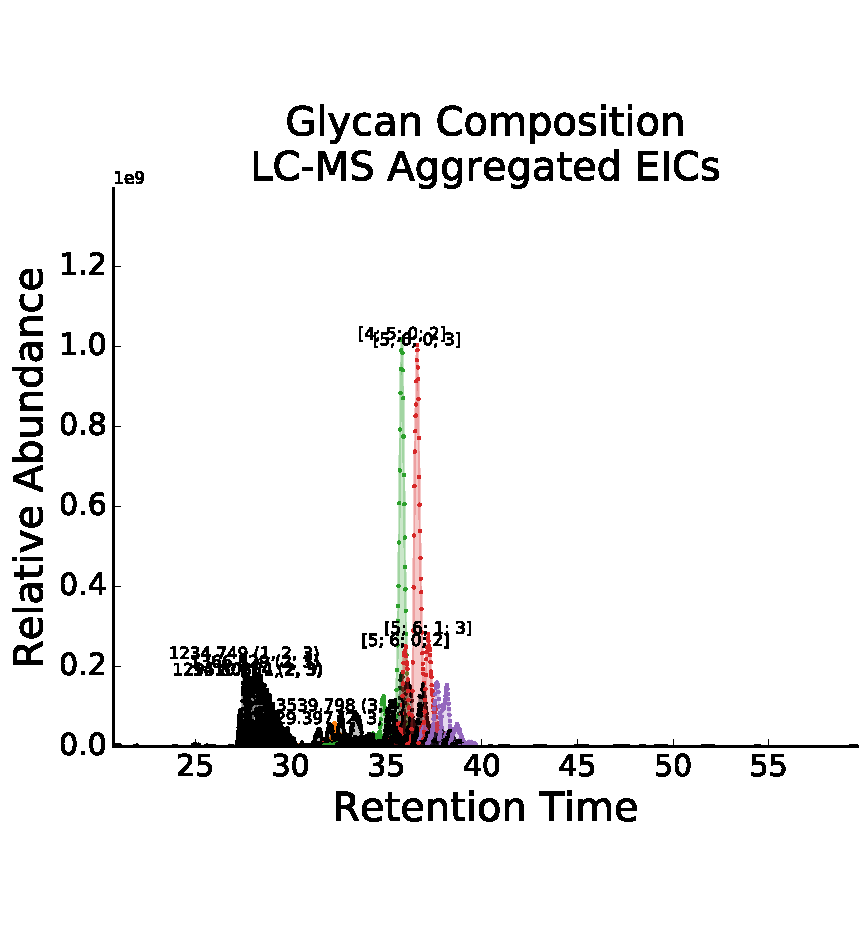
\includegraphics[width=0.45\textwidth,valign=t]{figure/rp_agp_chromatograms.pdf}
        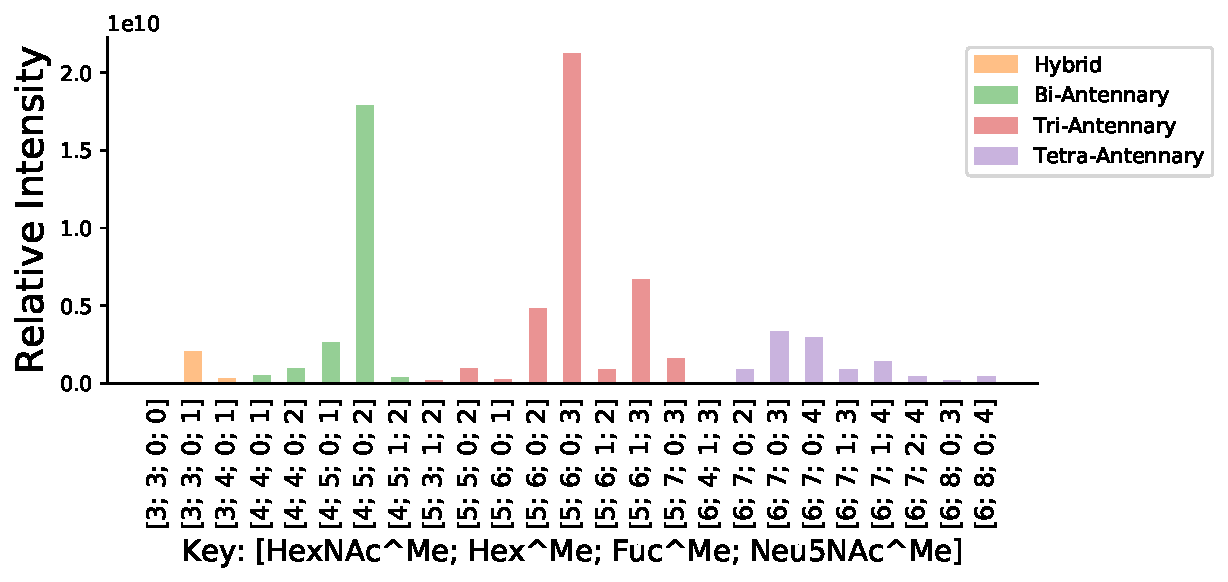
\includegraphics[width=0.45\textwidth,valign=t]{figure/rp_agp_abundances.pdf}
        \caption{\textit{AGP-permethylated-2ul-inj-55-SLens} Glycan Relative Abundances}
        \label{fig:rp_agp_aggregated_eics}
    \end{figure}

    \begin{table}
        \begin{minipage}[t]{0.25\linewidth}
            \vspace{0pt}
            (a)
            \centering
            
    \begin{tabular}{l | c}
        Group & $\tau$ \\
        \hline
        high-mannose & 0.00 \\
        hybrid & 20.22 \\
        bi-antennary & 18.50 \\
        asialo-bi-antennary & 14.15 \\
        tri-antennary & 21.33 \\
        asialo-tri-antennary & 11.71 \\
        tetra-antennary & 16.72 \\
        asialo-tetra-antennary & 1.43 \\
        penta-antennary & 8.13 \\
        asialo-penta-antennary & 0.00 \\
    \end{tabular}
    
            
        \end{minipage}
        \hspace{1cm}
        \begin{minipage}[t]{0.55\linewidth}
            \vspace{0pt}
            (b)
            \centering
            
    \begin{footnotesize}
    \begin{tabular}{l|p{2cm} p{2cm}}
Glycan Compostion &  Unregularized Score &  Regularized Score \\
\hline
\{Hex:3; HexNAc:3\}                   &                13.17 &              16.87 \\
\{Hex:3; HexNAc:3; Neu5NAc:1\}        &                20.04 &              18.03 \\
\{Hex:4; HexNAc:3; Neu5NAc:1\}        &                17.30 &              17.75 \\
\{Fuc:2; Hex:8; HexNAc:3\}            &                 5.85 &               1.01 \\
\{Fuc:1; Hex:9; HexNAc:3\}            &                 1.37 &               0.29 \\
\{Hex:4; HexNAc:4; Neu5NAc:1\}        &                19.72 &              17.30 \\
\{Hex:4; HexNAc:4; Neu5NAc:2\}        &                16.01 &              18.70 \\
\{Fuc:1; Hex:4; HexNAc:4; Neu5NAc:2\} &                 3.49 &               3.49 \\
\{Hex:5; HexNAc:4; Neu5NAc:1\}        &                22.71 &              17.63 \\
\{Hex:5; HexNAc:4; Neu5NAc:2\}        &                24.88 &              19.63 \\
\{Fuc:1; Hex:5; HexNAc:4; Neu5NAc:1\} &                15.95 &              16.71 \\
\{Fuc:1; Hex:5; HexNAc:4; Neu5NAc:2\} &                 7.21 &              17.51 \\
\{Hex:6; HexNAc:4; Neu5NAc:2\}        &                 3.53 &               3.53 \\
\{Fuc:3; Hex:6; HexNAc:4\}            &                 9.22 &              14.52 \\
\{Fuc:2; Hex:7; HexNAc:4; Neu5NAc:2\} &                  nan &              18.98 \\
\{Fuc:1; Hex:8; HexNAc:4; Neu5NAc:2\} &                 5.15 &               0.57 \\
\{Fuc:2; Hex:9; HexNAc:4; Neu5NAc:1\} &                 6.79 &               0.88 \\
\{Fuc:3; Hex:10; HexNAc:4\}           &                 8.29 &               1.65 \\
\{Fuc:1; Hex:3; HexNAc:5; Neu5NAc:2\} &                 7.96 &              16.94 \\
\{Hex:5; HexNAc:5; Neu5NAc:2\}        &                13.88 &              18.23 \\
\{Hex:6; HexNAc:5; Neu5NAc:1\}        &                 8.41 &              12.65 \\
\{Hex:6; HexNAc:5; Neu5NAc:2\}        &                21.65 &              18.71 \\
\{Hex:6; HexNAc:5; Neu5NAc:3\}        &                24.97 &              19.67 \\
\{Fuc:1; Hex:6; HexNAc:5; Neu5NAc:2\} &                11.26 &              17.89 \\
\{Fuc:1; Hex:6; HexNAc:5; Neu5NAc:3\} &                17.38 &              18.64 \\
\{Hex:7; HexNAc:5; Neu5NAc:3\}        &                15.78 &              18.73 \\
\{Hex:7; HexNAc:6; Neu5NAc:2\}        &                10.36 &              15.41 \\
\{Hex:7; HexNAc:6; Neu5NAc:3\}        &                16.80 &              16.03 \\
\{Hex:7; HexNAc:6; Neu5NAc:4\}        &                18.28 &              16.26 \\
\{Fuc:1; Hex:7; HexNAc:6; Neu5NAc:2\} &                 9.17 &              15.42 \\
\{Fuc:1; Hex:7; HexNAc:6; Neu5NAc:3\} &                14.56 &              15.85 \\
\{Fuc:1; Hex:7; HexNAc:6; Neu5NAc:4\} &                19.27 &              16.17 \\
\{Fuc:2; Hex:7; HexNAc:6; Neu5NAc:3\} &                 9.60 &              15.34 \\
\{Fuc:2; Hex:7; HexNAc:6; Neu5NAc:4\} &                10.14 &              15.08 \\
\{Hex:8; HexNAc:6; Neu5NAc:3\}        &                 8.75 &              12.08 \\
\{Hex:8; HexNAc:6; Neu5NAc:4\}        &                 9.87 &              11.96 \\
\{Fuc:1; Hex:8; HexNAc:6; Neu5NAc:4\} &                 5.50 &              11.58 \\
\{Hex:9; HexNAc:7\}                   &                 4.48 &                nan \\
\end{tabular}

    \end{footnotesize}
    
        \end{minipage}
        \caption{
                 Search Results for \textit{AGP-permethylated-2ul-inj-55-SLens}.
                 (a) Estimated $\mathbf{\tau}$ for grid with ${\hat \gamma} = 16.167868$.
                 (b) Scores For Identified Glycans of grid with ${\hat \lambda} = 0.99$.}
        \label{tbl:rp_agp_score_table}
    \end{table}
